
\section{Discrete Kalman Filter} \label{sec:part5}
In this part a discrete Kalman filter is implemented to estimate the bias b and the heading $\psi$. The high-frequented wave induced motion $\psi_m$ is also estimated, but this must be removed from the control loop to avoid wear and tear on the actuator system. We continue to be careful not to make $\psi$ bigger than $\pm 35 \circ$ and small deviations in compass value. Our saturation is on the input of the system, which may be interpreted as it is the rudder input rather than the head that is saturated. \todo{husk å nevne i d og e}
\medskip
Kalman filtering applies a recursive method for estimation of a random process. The optimization criterion used is minimization of the mean-squared estimation error of the random variable x.

\subsection{Exact discretization}
To use a discrete Kalman filter, a discretized system is needed. The matrices A, B and E found in \ref{sec:part4-1} was put into Matlab and the function \texttt{c2d} with sampling frequency of 10 Hz was used to get an exact discretization of the system $A_d$, $B_d$ and $E_d$ (see code below). The \texttt{c2d} function uses zero-order hold to get a discrete counterpart to the continous system, and had to be used twice as the function only discretize two matrices at the time. The matrices $C_d$ and $D_d$ are the same as C and D as shown in page 110 in \cite{chen14}.
\lstinputlisting{Matlabkode/p5_a.m}


\subsection{Estimate of measurement noise variance}\label{eq:noise_vaiance}
To find the estimate of the variance of the measurement noise we used the Matlab function \texttt{var} on the measured compass course. This data was imported from Matlab and transformed from degrees to radians before taking the mean variance. The variance was found to be $ = 6.0813*10^{-7}$.
\lstinputlisting{Matlabkode/p5_b.m}



\subsection{Implementation of discrete Kalman filter}
To implement the discrete Kalman filter we chose to use a Matlab function block in Simulink. To initialize the filter the following was given from the assignment
\begin{equation}
    \boldsymbol{w} = [w_w \ w_b]^T \ , \ E\{\boldsymbol{w w^T}\} = \boldsymbol{Q} = \begin{bmatrix}
        30 & 0 \\
        0 & 10^{-6} 
    \end{bmatrix}
\end{equation}

\begin{equation}
    \boldsymbol{P_0^-} = \begin{bmatrix}
        1 & 0 & 0 & 0 & 0 \\
        0 & 0.013 & 0 & 0 & 0 \\
        0 & 0 & \pi^2 & 0 & 0 \\
        0 & 0 & 0 & 1 & 0 \\
        0 & 0 & 0 & 0 & 2.5 \cdot 10^{-3} 
    \end{bmatrix} \ , \ \boldsymbol{x_0^-} = \begin{bmatrix}
        0 \\ 0 \\ 0 \\ 0 \\ 0 \\
    \end{bmatrix}
\end{equation}
\textbf{w} is the process noise, \textbf{Q} is the process noise covariance, $\boldsymbol{\hat{x}_0^-}$ is the initial a priori state estimate and $\boldsymbol{P_0^-}$ is the initial a priori estimate error covariance. $E(v^2) = R = \frac{variance}{T_{s}}$ where the variance was found in the previous section and $T_{s}$ was $\frac{1}{F_s}$. This is because the process is sampled.
\newline\newline
Now with the initial phase defined the equations from \cite{chen14} was used to create the Kalman filter. The first step of the Kalman filter is to calculate the new Kalman gain, K.
\begin{equation}
    K = \boldsymbol{P^-}\boldsymbol{C}_d^T(\boldsymbol{C}_d\boldsymbol{P^-}\boldsymbol{C}_d^T+R)^{-1};
\end{equation}
With this new gain it is now possible to move to the second step which is to update to our new state $\boldsymbol{\hat{x}}$ and our new estimate error covariance $\boldsymbol{P}$, also known as  $\boldsymbol{\hat{x}}$ and $\boldsymbol{P}$ a posteriori. The y used here is the measured compass course.
\begin{equation}
    \boldsymbol{\hat{x}} = \boldsymbol{\hat{x}^-} + K(\boldsymbol{y}-\boldsymbol{C}_d\boldsymbol{\hat{x}^-})
\end{equation}
\begin{equation}
    \boldsymbol{P} = (\boldsymbol{I}-\boldsymbol{K}\boldsymbol{C}_d)\boldsymbol{P^-}(\boldsymbol{I}-\boldsymbol{K}\boldsymbol{C}_d)^T+KRK^T;
\end{equation}
The third step is to project ahead and create what will become the new $\boldsymbol{x}$ and $\boldsymbol{P}$ a priori.
\begin{equation}
    \boldsymbol{\hat{x}}^-_{k+1} = \boldsymbol{A_d}\boldsymbol{\hat{x}} + \boldsymbol{B_d}u
\end{equation}
\begin{equation}
    \boldsymbol{\hat{P}}^-_{k+1} = \boldsymbol{A_d}\boldsymbol{P}\boldsymbol{A_d}^T + \boldsymbol{Ed}\boldsymbol{Q}\boldsymbol{E_d}^T;
\end{equation}
All of these functions plus the initialization was implemented in Matlab as seen below. The new estimated compass course $\psi$, here called y$\_$est, and the bias b was updated at the end to be used in the controll loop. The Simulink implementation of this part can be seen in \ref{sim:part5c}.Here a \textit{Zero Order Hold} block was used to make the signal discrete. This was necessary to do since the design was a discrete Kalman filter. \newline
The Kalman filter depends on the control input, but the input of the Kalman filter depemnds on the output for the Kalman filter. This does that Simulink is not able to determan the initial values and blame on an \textit{algebraic loop}. This is solved by adding a \textit{Memory} block on the output of the Kalman filter.  

%\inputminted[linenos]{Matlab}{Part5_pics/p5_Kalman.m}
\begin{figure}[H]
    \centering
    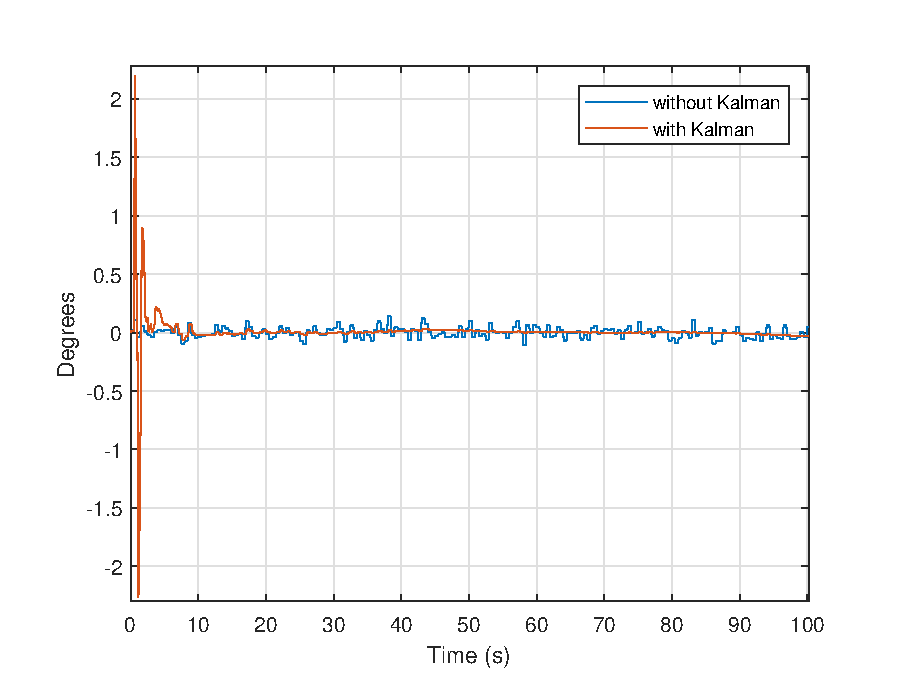
\includegraphics[width=0.8\linewidth]{Part5_pics/ny_p5c.eps}
    \caption{Signal with and without Kalman filtering }
    \label{fig:p5c}
\end{figure}
si litt om hvorfor vi får så høye verdier på kalman filteret. jeh tror det er pga filteret trenger noen runder til p feile seg til riktig verdi. eller skal vi droppe bilde?? 
må vel også nevnes at kalman filteret er diuskret mens modellen er kontinuelig. 


\subsection{Simulation with current disturbance with feed forward}
For testing the Kalman filter and the performance of the autopilot a simulation with $\psi_r = 30$ was used. The figure \ref{fig:p5d} shows the values in the simulation. 
\newline
\begin{figure}[H]
    \centering
    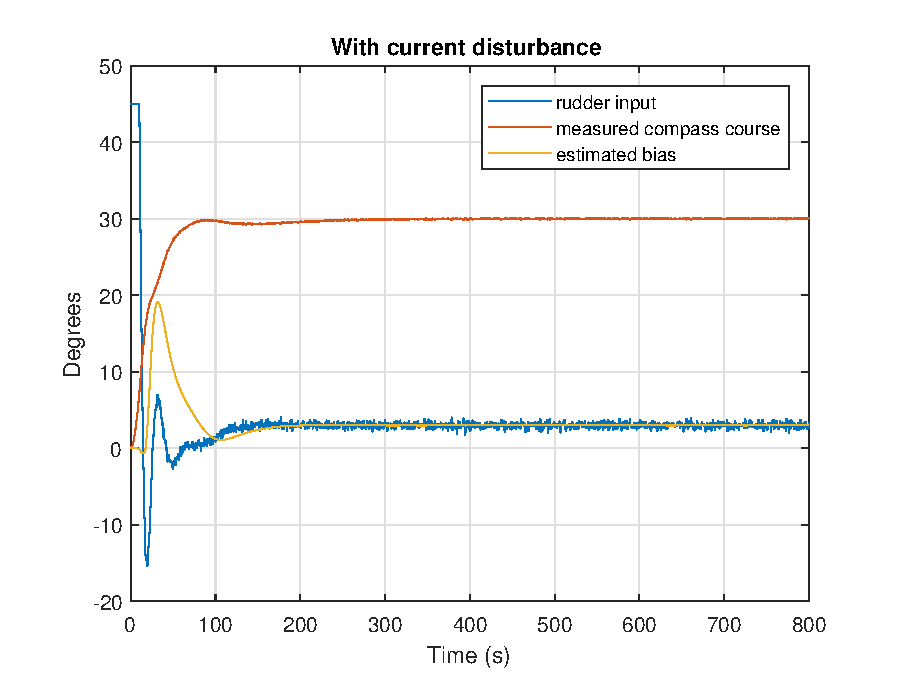
\includegraphics[width=0.8\linewidth]{Part5_pics/ny_p5d.eps}
    \caption{Autopilot with Kalman filtering and current disturbance}
    \label{fig:p5d}
\end{figure}
The biggest defence is that the compass course contains 30 degrees. 
This is because the rudder bias that is estimates is accurate enough to cancel out the real rudder bias. Hence, we have a better performance of the autopilot then in section \ref{p3c}. 



\subsection{Simulation with wave and current disturbance and wave filtering}
In this subsection we are simulatin with both wave and current disturbance. Instead of the measured compass couse we use the wave filtered $\psi$ signal.  
\newline
\begin{figure}[H]
    \centering
    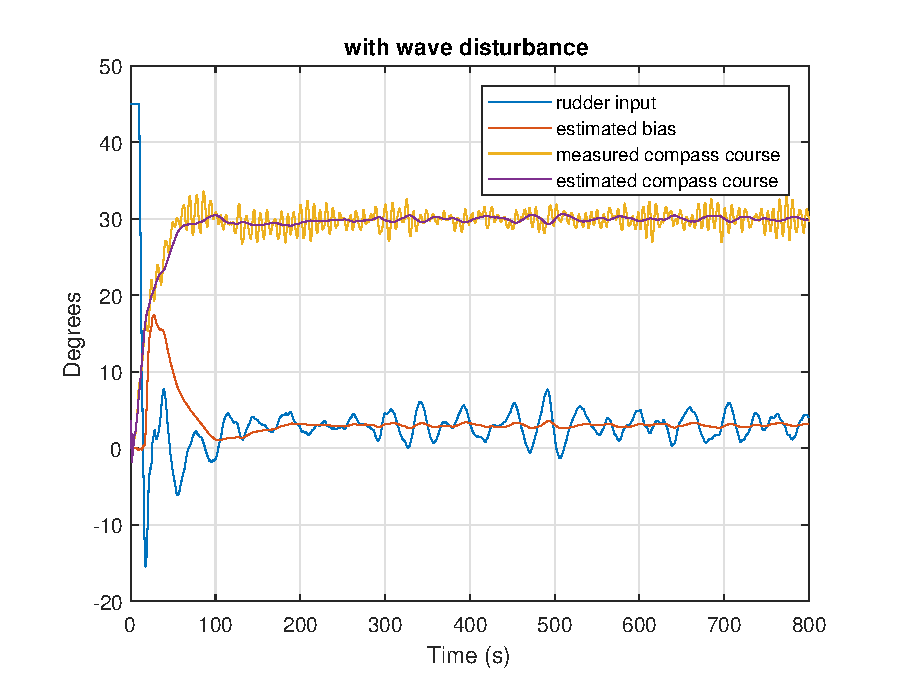
\includegraphics[width=0.8\linewidth]{Part5_pics/ny_p5e.eps}
    \caption{Autopilot with Kalman filtering with wave and current disturbance}
    \label{fig:p5e}
\end{figure}
In figure \ref{fig:p5e} is the simulation with wave and current disturbance. A big difference from the autopilot in section \ref{p3d} is that the rudder input does not fluctuate as much. This is a desirable because the system would must likely be less damaged by the oscillation.\newline 
The estimated compass course is the filtered compass course from the Kalman filter, we see here that the signal is better that without the Kalman filter.\newline 
An alternative could we using a low-pass filter on the compass measurement. This would probably removed some of the $\psi_\omega$, but not the wave disturbance.  The conclusion is that with the Kalman filter we get a mot robust and reliable system. 
\bigskip
In figure.. ett eller annent can we compare the actual wave influence and estimated wave influence. 